\newcommand\skipCaption[1]{
  \vspace*{-6mm}
  \caption{#1}
}

\newcommand\skipCaptionA[2]{
  \vspace*{-#1mm}
  \caption{#2}
}

\chapter{Resultaten}
\label{hoofdstuk:resultaten}
Dit hoofdstuk bespreekt de resultaten van de nieuwe $\symBSPsweep$ bomen.
In sectie \ref{h5:praktische-aspecten} worden een aantal praktische aspecten omtrent de testopstelling besproken zoals de scenes, de gebruikte parameters en het gebruikte computersysteem.
Daarna bespreken we de invloed van het aantal richtingen op de vorm (sectie \ref{h5-richtingen-bespreking}) en kwaliteit (sectie \ref{h5-richtingen-kwaliteit}) van de negen soorten $\symBSPsweep$ bomen.
De laatste sectie (sectie \ref{h5-vergelijken}) vergelijkt de beste $\symBSPsweep$ bomen met de bomen besproken in hoofdstuk \ref{hoofdstuk:voorgaand-werk}.

\section{Praktische aspecten}
\label{h5:praktische-aspecten}
Alle $\symBSP$ bomen zijn geïmplementeerd in het pbrt framework zoals besproken in hoofdstuk \ref{hoofdstuk:implementatie}. 
Dit framework maakt geen gebruik van optimalisaties zoals SIMD instructies en de GPU. 
Hierdoor kan de kracht van de verschillende bomen objectief vergeleken worden.\\

Figuur \ref{fig:results-scenes} toont de gebruikte testscenes en tabel \ref{tab:results-statistics-scenes} toont informatie over deze scenes.
De Killeroo Been scene is een scene waarbij algemene $\symBSP$ bomen voordeel hebben ten opzichte van de $\symKd$ boom omwille van de complexe geometrie waarop is ingezoomd.
De drie andere scenes zijn realistische indoor scenes.
Alle scenes maken gebruik van Halton sampling met een specifiek aantal stralen per pixel \textit{spp}.
De globale belichting wordt berekend via \textit{path tracing} waarbij steeds een maximale diepte van 5 gebruikt wordt, behalve bij de museum scene waar enkel directe belichting gebruikt wordt.\\

\begin{figure}
  \begin{subfigure}[t]{0.25\textwidth}
    \centering
    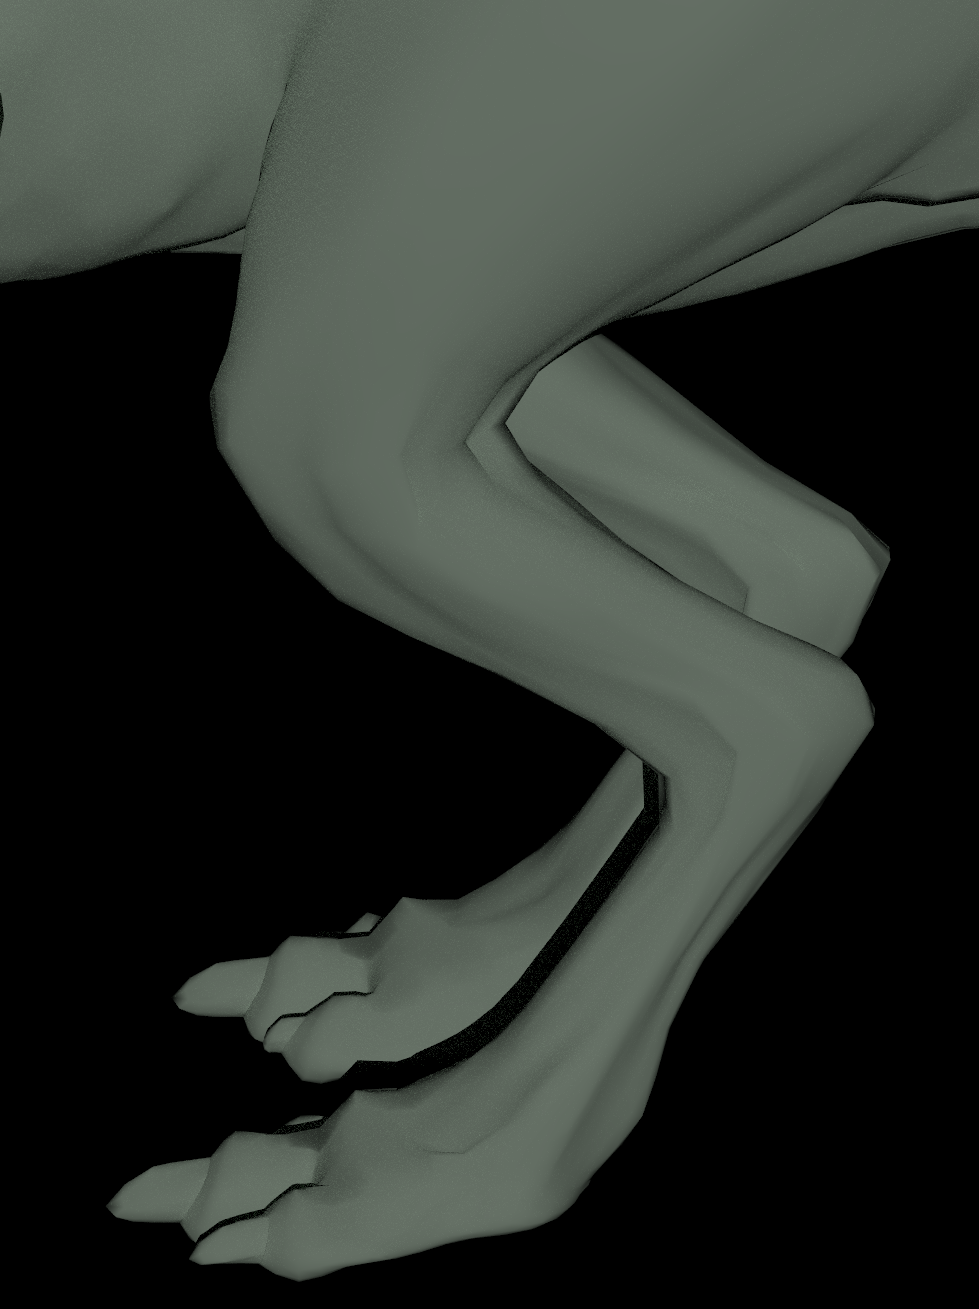
\includegraphics[width=0.6\linewidth]{img/killerooFeet}
    \caption{Killeroo Been scene}
    \label{fig:results-scene-killeroo-been}    
  \end{subfigure}
  \begin{subfigure}[t]{0.20\textwidth}
    \centering
    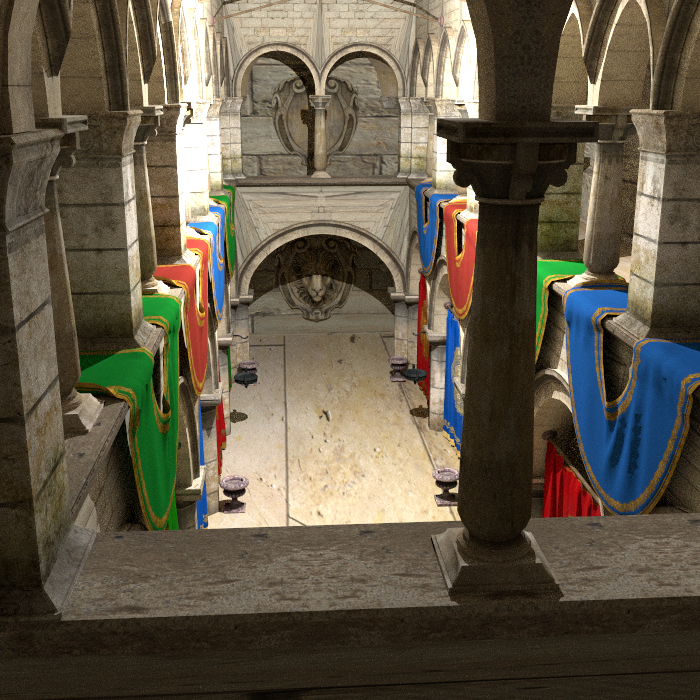
\includegraphics[width=1\linewidth]{img/sponza}
    \caption{Sponza scene}
    \label{fig:results-scene-sponza}    
  \end{subfigure}
  \begin{subfigure}[t]{0.29\textwidth}
    \centering
    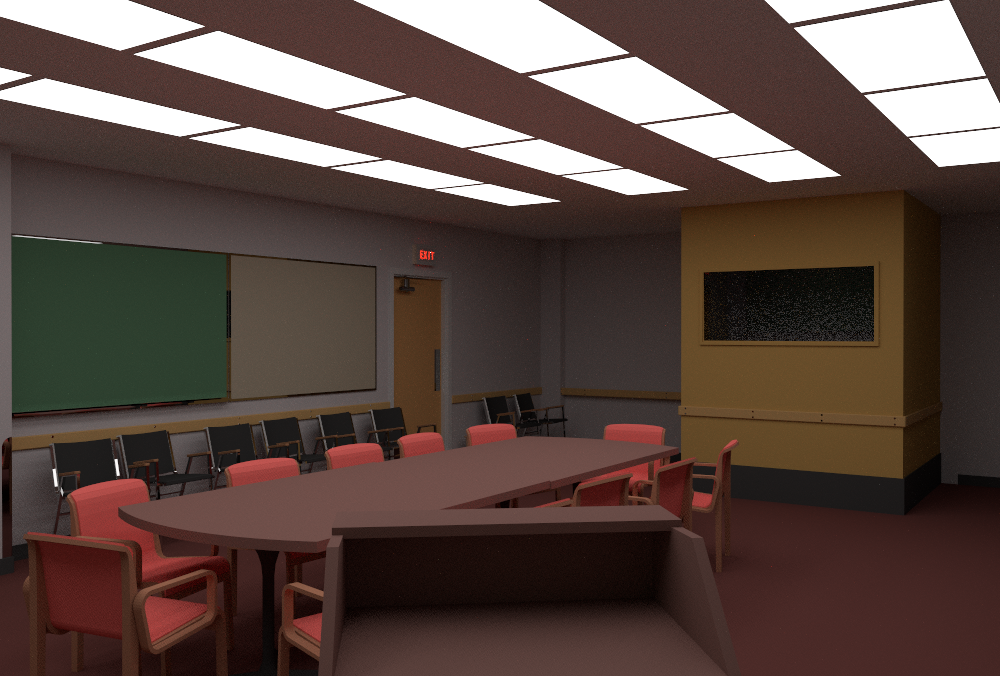
\includegraphics[width=1\linewidth]{img/conferencehall}
    \caption{Conference scene}
    \label{fig:results-scene-conference}    
  \end{subfigure}
  \begin{subfigure}[t]{0.20\textwidth}
    \centering
    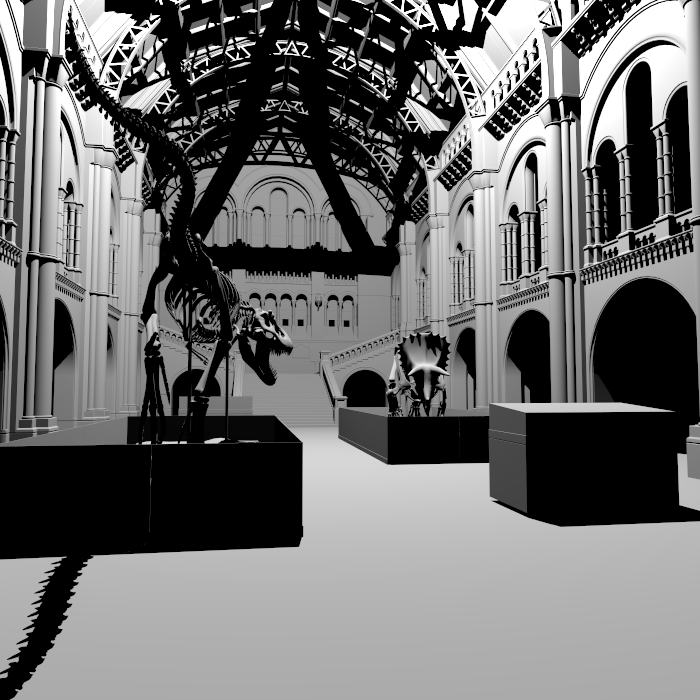
\includegraphics[width=1\linewidth]{img/museum}
    \caption{Museum scene}
    \label{fig:results-scene-museum}    
  \end{subfigure}
  \caption[Testscenes]{Testscenes - \small De testscenes gebruikt om de nieuwe $\symBSP$ te testen}
  \label{fig:results-scenes}
\end{figure}

\begin{table}
  \centering
  \begin{tabular}{@{}lcccc@{}} \toprule
  Scene & Aantal driehoeken & Resolutie & Sampling per pixel & Belichting\\ \midrule
  Killeroo Been & 33264 & 5000x5000 & Halton, 8spp & \textit{path tracing}, diepte 5\\
  Sponza & 227309 & 700x700 & Halton, 64spp & \textit{path tracing}, diepte 5\\
  Conference & 123651 & 1000x676 & Halton, 64spp & \textit{path tracing}, diepte 5\\
  Museum & 1462840 & 700X700 & Halton, 64spp & \textit{path tracing}, diepte 1\\ \bottomrule
 \end{tabular}
  \caption[Statistieken Testscenes]{Statistieken Testscenes - \small Statistieken van de testscenes gebruikt om de nieuwe $\symBSP$ te testen}
  \label{tab:results-statistics-scenes}
\end{table}

Tabel \ref{tab:results-parameters} toont de parameterwaarden die gebruikt zijn bij de testen. De formule voor de maximale diepte is afhankelijk van het aantal driehoeken n en is bedacht door \authorHavranBittner{} \cite{havran2002improving} voor $\symKd$ bomen. Deze parameterwaarden zijn niet geoptimaliseerd en kunnen mogelijks beter worden afgesteld.
De specificaties van het gebruikte computersysteem worden getoond in figuur \ref{tab:results-specs}.
\begin{table}
  \centering
  \begin{tabular}{@{}lc@{}} \toprule
  Parameter & Waarde \\ \midrule
  $\symCost_\symIntersection$ & 80 \\
  $\symCostTraversalKd$ & 1 \\
  $\symCostTraversalBSP$ & 5 \\
  $\symMaxPrims$ & 1 \\
  $\symMaxDepth$ & $k1log_2(n) + k2$ met $k1 = 1.6$ en $k2 = 2$ \\
  \bottomrule
 \end{tabular}
  \caption[Gebruikte parameterwaarden]{Gebruikte parameterwaarden - \small De waarden voor de parameters gebruikt om de nieuwe $\symBSP$ te testen}
  \label{tab:results-parameters}
\end{table}

\begin{table}
  \centering
  \begin{tabular}{@{}lc@{}} \toprule
  Parameter & Waarde \\ \midrule
  CPU & Intel Core i7-6700HQ CPU @ 2.60GHz x 8 \\
  Geheugen & 16 GB DDR4 \\
  Besturingssysteem & Ubuntu 18.04.2 LTS 64-bit \\
  \bottomrule
 \end{tabular}
  \caption[Specificaties computersysteem]{Specificaties computersysteem - \small De specificaties van het gebruikte computersysteem.}
  \label{tab:results-specs}
\end{table}

\newcommand{\plotVsK}[5] {
  \begin{tikzpicture}[scale=0.5]
    \begin{axis}[
      axis lines = left,
      ylabel = #5,
      xlabel = K,
      ymin=#3, ymax=#4,
      width=1.8\textwidth,
      height=2.2\textwidth,
      cycle multi list={%
        color list\nextlist
        [3 of]mark list
      },
      legend style={at={(0.5,-0.15)}, anchor=north,legend columns=3},
      title = #2,
  ]
    \addplot table [x=K, y=#1, col sep=comma] {data/bsprandomRender.csv};
    \addlegendentry{$\symBSPrandom$}
    \addplot table [x=K, y=#1, col sep=comma] {data/bsprandomwithkdRender.csv};
    \addlegendentry{$\symBSPrandomkd$}
    \addplot table [x=K, y=#1, col sep=comma] {data/bsprandomfastkdRender.csv};
    \addlegendentry{$\symBSPrandomfastkd$}
    
    \addplot table [x=K, y=#1, col sep=comma] {data/bsparbitraryRender.csv};
    \addlegendentry{$\symBSParbitrary$}
    \addplot table [x=K, y=#1, col sep=comma] {data/bsparbitrarywithkdRender.csv};
    \addlegendentry{$\symBSParbitrarykd$}
    \addplot table [x=K, y=#1, col sep=comma] {data/bsparbitraryfastkdRender.csv};
    \addlegendentry{$\symBSParbitraryfastkd$}
    
    \addplot table [x=K, y=#1, col sep=comma] {data/bspclusterRender.csv};
    \addlegendentry{$\symBSPcluster$}
    \addplot table [x=K, y=#1, col sep=comma] {data/bspclusterwithkdRender.csv};
    \addlegendentry{$\symBSPclusterkd$}
    \addplot table [x=K, y=#1, col sep=comma] {data/bspclusterfastkdRender.csv};
    \addlegendentry{$\symBSPclusterfastkd$}
      \end{axis}
    \end{tikzpicture}
}

\newcommand{\plotFastKdVsK}[5] {
  \begin{tikzpicture}[scale=0.5]
    \begin{axis}[
      axis lines = left,
      ylabel = #5,
      xlabel = K,
      ymin=#3, ymax=#4,
      width=1.8\textwidth,
      height=2.2\textwidth,
      cycle multi list={%
        color list\nextlist
        mark=triangle*
      },
      legend style={at={(0.5,-0.15)}, anchor=north,legend columns=3},
      title = #2,
  ]
    
    \addplot table [x=K, y=#1, col sep=comma, mark=diamond*] {data/bsprandomfastkdRender.csv};
    \addlegendentry{$\symBSPrandomfastkd$}
    
    \addplot table [x=K, y=#1, col sep=comma, mark=diamond*] {data/bsparbitraryfastkdRender.csv};
    \addlegendentry{$\symBSParbitraryfastkd$}
    
    \addplot table [x=K, y=#1, col sep=comma, mark=diamond*] {data/bspclusterfastkdRender.csv};
    \addlegendentry{$\symBSPclusterfastkd$}
      \end{axis}
    \end{tikzpicture}
}

\newcommand{\plotRendertimeKScenes}[4] {
  \begin{tikzpicture}
    \begin{axis}[
      axis lines = left,
      ylabel = Procentuele tijd tov de $\symKd$ boom,
      xlabel = K,
      ymin=#3, ymax=#4,
      width=0.5\textwidth,
      height=0.8\textwidth,
      %cycle multi list={%
      %  color list\nextlist
      %  [3 of]mark list
      %},
      title = #2,
      legend pos=north east,
  ]
    \addplot table [x=K, y=RendertimeTovKdFeet, col sep=comma] {#1};
    \addlegendentry{Med Killeroo Been}
    \addplot table [x=K, y=RendertimeTovKdSponza, col sep=comma] {#1};
    \addlegendentry{Med Sponza Been}
    \addplot table [x=K, y=RendertimeTovKdConference, col sep=comma] {#1};
    \addlegendentry{Med Conference Been}
    
      \end{axis}
    \end{tikzpicture}
}
\newcommand{\plotSAKScenes}[4] {
  \begin{tikzpicture}
    \begin{axis}[
      axis lines = left,
      ylabel = Procentuele SA tov de $\symKd$ boom,
      xlabel = K,
      ymin=#3, ymax=#4,
      width=0.5\textwidth,
      height=0.8\textwidth,
      %cycle multi list={%
      %  color list\nextlist
      %  [3 of]mark list
      %},
      title = #2,
      legend pos=north east,
  ]
    \addplot table [x=K, y=SATovKdFeet, col sep=comma] {#1};
    \addlegendentry{Killeroo Been}
    \addplot table [x=K, y=SATovKdSponza, col sep=comma] {#1};
    \addlegendentry{Sponza Been}
    \addplot table [x=K, y=SATovKdConference, col sep=comma] {#1};
    \addlegendentry{Conference Been}
    
      \end{axis}
    \end{tikzpicture}
}
\newcommand{\plotPrimIntBothKScenes}[4] {
  \begin{tikzpicture}
    \begin{axis}[
      axis lines = left,
      ylabel = Procentueel aantal intersecties tov de $\symKd$ boom,
      xlabel = K,
      ymin=#3, ymax=#4,
      width=0.5\textwidth,
      height=0.8\textwidth,
      cycle multi list={%
        color list\nextlist
        [2 of]mark list
      },
      title = #2,
      legend pos=north east,
  ]
    \addplot table [x=K, y=nbPrimIntTovKdFeet, col sep=comma] {#1};
    \addlegendentry{Prim Killeroo Been}    
    \addplot table [x=K, y=nbPrimIntPTovKdFeet, col sep=comma] {#1};
    \addlegendentry{Sec Killeroo Been}
    
    \addplot table [x=K, y=nbPrimIntTovKdSponza, col sep=comma] {#1};
    \addlegendentry{Prim Sponza Been}    
    \addplot table [x=K, y=nbPrimIntPTovKdSponza, col sep=comma] {#1};
    \addlegendentry{Sec Sponza Been}
    
    \addplot table [x=K, y=nbPrimIntTovKdConference, col sep=comma] {#1};
    \addlegendentry{Prim Conference Been}
    \addplot table [x=K, y=nbPrimIntPTovKdConference, col sep=comma] {#1};
    \addlegendentry{Sec Conference Been}
    
      \end{axis}
    \end{tikzpicture}
}
\newcommand{\plotTravBothKScenes}[4] {
  \begin{tikzpicture}
    \begin{axis}[
      axis lines = left,
      ylabel = Procentueel aantal doorkruisingen tov de $\symKd$ boom,
      xlabel = K,
      ymin=#3, ymax=#4,
      width=0.5\textwidth,
      height=0.8\textwidth,
      cycle multi list={%
        color list\nextlist
        [2 of]mark list
      },
      title = #2,
      legend pos=outer north east,
  ]
    \addplot table [x=K, y=nbNodeTravTovKdFeet, col sep=comma] {#1};
    \addlegendentry{Prim Killeroo Been}    
    \addplot table [x=K, y=nbNodeTravPTovKdFeet, col sep=comma] {#1};
    \addlegendentry{Sec Killeroo Been}
    
    \addplot table [x=K, y=nbNodeTravTovKdSponza, col sep=comma] {#1};
    \addlegendentry{Prim Sponza Been}    
    \addplot table [x=K, y=nbNodeTravPTovKdSponza, col sep=comma] {#1};
    \addlegendentry{Sec Sponza Been}
    
    \addplot table [x=K, y=nbNodeTravTovKdConference, col sep=comma] {#1};
    \addlegendentry{Prim Conference Been}
    \addplot table [x=K, y=nbNodeTravPTovKdConference, col sep=comma] {#1};
    \addlegendentry{Sec Conference Been}
    
      \end{axis}
    \end{tikzpicture}
}
\newcommand{\plotKdTravProcBothKScenes}[4] {
  \begin{tikzpicture}
    \begin{axis}[
      axis lines = left,
      ylabel = Procentueel aantal $\symKd$ doorkruisingen,
      xlabel = K,
      ymin=#3, ymax=#4,
      width=0.5\textwidth,
      height=0.8\textwidth,
      cycle multi list={%
        color list\nextlist
        [2 of]mark list
      },
      title = #2,
      legend pos=outer north east,
  ]
    \addplot table [x=K, y=nbKdNodeTravPercFeet, col sep=comma] {#1};
    \addlegendentry{Prim Killeroo Been}    
    \addplot table [x=K, y=nbKdNodeTravPPercFeet, col sep=comma] {#1};
    \addlegendentry{Sec Killeroo Been}
    
    \addplot table [x=K, y=nbKdNodeTravPercSponza, col sep=comma] {#1};
    \addlegendentry{Prim Sponza Been}    
    \addplot table [x=K, y=nbKdNodeTravPPercSponza, col sep=comma] {#1};
    \addlegendentry{Sec Sponza Been}
    
    \addplot table [x=K, y=nbKdNodeTravPercConference, col sep=comma] {#1};
    \addlegendentry{Prim Conference Been}
    \addplot table [x=K, y=nbKdNodeTravPPercConference, col sep=comma] {#1};
    \addlegendentry{Sec Conference Been}
    
      \end{axis}
    \end{tikzpicture}
}
\newcommand{\plotKdNodeProcBothKScenes}[4] {
  \begin{tikzpicture}
    \begin{axis}[
      axis lines = left,
      ylabel = Procentueel aantal $\symKd$ knopen,
      xlabel = K,
      ymin=#3, ymax=#4,
      width=0.5\textwidth,
      height=0.8\textwidth,
      cycle multi list={%
        color list\nextlist
        [1 of]mark list
      },
      title = #2,
      legend pos=outer north east,
  ]
    \addplot table [x=K, y=nbKdNodePercFeet, col sep=comma] {#1};
    \addlegendentry{Killeroo Been}   
    
    \addplot table [x=K, y=nbKdNodePercSponza, col sep=comma] {#1};
    \addlegendentry{Sponza Been}    
    
    \addplot table [x=K, y=nbKdNodePercConference, col sep=comma] {#1};
    \addlegendentry{Prim Conference Been}
    
      \end{axis}
    \end{tikzpicture}
}
\newcommand{\plotBuildtimeKScenes}[4] {
  \begin{tikzpicture}
    \begin{axis}[
      axis lines = left,
      ylabel = Bouwtijd in seconden,
      xlabel = K,
      %ymin=#3, ymax=#4,
      width=0.5\textwidth,
      height=0.8\textwidth,
      %cycle multi list={%
      %  color list\nextlist
      %  [3 of]mark list
      %},
      title = #2,
      legend pos=north east,
  ]
    \addplot table [x=K, y=BuildtimeFeet, col sep=comma] {#1};
    \addlegendentry{Med Killeroo Been}
    \addplot table [x=K, y=BuildtimeSponza, col sep=comma] {#1};
    \addlegendentry{Med Sponza Been}
    \addplot table [x=K, y=BuildtimeConference, col sep=comma] {#1};
    \addlegendentry{Med Conference Been}
    
      \end{axis}
    \end{tikzpicture}
}
\newcommand{\plotBuildtimeTovKdKScenes}[4] {
  \begin{tikzpicture}
    \begin{axis}[
      axis lines = left,
      ylabel = Bouwtijd in seconden,
      xlabel = K,
      %ymin=#3, ymax=#4,
      width=0.5\textwidth,
      height=0.8\textwidth,
      %cycle multi list={%
      %  color list\nextlist
      %  [3 of]mark list
      %},
      title = #2,
      legend pos=north east,
  ]
    \addplot table [x=K, y=BuildtimeTovKdFeet, col sep=comma] {#1};
    \addlegendentry{Med Killeroo Been}
    \addplot table [x=K, y=BuildtimeTovKdSponza, col sep=comma] {#1};
    \addlegendentry{Med Sponza Been}
    \addplot table [x=K, y=BuildtimeTovKdConference, col sep=comma] {#1};
    \addlegendentry{Med Conference Been}
    
      \end{axis}
    \end{tikzpicture}
}
%\plotRendertimeK{renderMinKdFeet}{Minimale tijd Killeroo Been}
%\plotRendertimeK{renderMaxKdFeet}{Maximale tijd Killeroo Been}

\section{Afhankelijkheid van aantal richtingen}
In deze sectie wordt de afhankelijkheid van $\symBSPsweep$ bomen van het aantal gebruikte richtingen k, besproken. 
Alle negen varianten hebben bovenstaande scenes zeven keer gerenderd voor k-waarden van 2 tot en met 10.
De zes varianten die gebruik maken van de $\symKd$ richtingen, moeten altijd een k waarde van minstens 3 hebben, dus deze zijn niet gerenderd voor $k = 2$.
Voor elke combinatie van $\symBSP$ boom en k-waarde wordt de uitvoering waarvan de rendertijd gelijk is aan de mediaan van de rendertijden van de zeven uitvoeringen, gebruikt als representatieve uitvoering.
Alle onderstaande analyses maken gebruik van die uitvoeringen.
\subsection{Bespreking bomen}
\label{h5-richtingen-bespreking}
\paragraph{Bouwtijd} Figuur \ref{fig:k-bouwtijd} toont de bouwtijden ten opzichte van de bouwtijden van de $\symKd$ boom. De bouwtijden van de $\symBSPsweep$ bomen zijn twee ordergroottes groter dan die van de $\symKd$ boom. De grafieken voor de verschillende scenes (met een verschillend aan driehoeken) zijn zeer gelijkaardig, dus is de complexiteit voor het bouwen van $\symKd$ en $\symBSPsweep$ bomen op dezelfde manier afhankelijk van het aantal driehoeken. De grafieken van de $\symBSPrandom$ bomen zijn alle drie bijna perfecte rechten. De bouwtijd is lineair afhankelijk van k omdat in elke knoop over k richtingen gesweept wordt. Bij de $\symBSParbitrary$ en $\symBSPcluster$ bomen is de afhankelijkheid sublineair omdat er in knopen met minder dan k driehoeken, over minder dan k richtingen gesweept wordt. 
De $\symBSPrandomfastkd$, $\symBSParbitraryfastkd$ en $\symBSPclusterfastkd$ bomen met $k = 3$ zijn identiek aan de $\symKd$ boom, maar gebouwd met convexe veelvlakken in plaats van asgealigneerde balken.
Hieruit kunnen we afleiden dat het gebruik van convexe veelvlakken tijdens het bouwen ongeveer 25 (2500\%) keer trager is dan het gebruik van asgealigneerde balken.
\begin{figure}[h]
  \centering
  \begin{subfigure}[t]{.32\linewidth}
    \centering
\plotVsK{BuildtimeTovKdFeet}{}{2000}{26000}{Procentuele bouwtijd tov de $\symKd$ boom}
  \skipCaptionA{4}{Killeroo Been}
  \end{subfigure}
  \begin{subfigure}[t]{.32\linewidth}
    \centering
\plotVsK{BuildtimeTovKdSponza}{}{2000}{26000}{Procentuele bouwtijd tov de $\symKd$ boom}
\skipCaptionA{4}{Sponza}
\end{subfigure}
\begin{subfigure}[t]{.32\linewidth}
  \centering
\plotVsK{BuildtimeTovKdConference}{}{2000}{26000}{Procentuele bouwtijd tov de $\symKd$ boom}
\skipCaptionA{4}{Conference}
\end{subfigure}
\caption[Bouwtijd in functie van k]{Bouwtijd in functie van k - \small Deze grafieken tonen voor elke scene de procentuele bouwtijd van de $\symBSPsweep$ bomen ten opzichte van de bouwtijd van de $\symKd$ boom in functie van k.}
\label{fig:k-bouwtijd}
\end{figure}


\paragraph{$\mathbf{\symSAH}$}
De $\symSAH$ wordt gebruikt om in elke knoop op een greedy manier het beste splitsingsvlak te bepalen. De totale $\symSAH$ kost van de boom kan echter ook berekend worden. Bij de $\symBSPsweep$ bomen die gebruik maken van $\symKd$ richtingen, maar deze behandelen als $\symBSP$ vlakken, wordt $\symCostTraversalBSP$ gebruikt als doorkruiskost. Bij de $\symBSPsweepkd$ bomen wordt de $\symCostTraversalKd$ gebruikt als doorkruiskost voor de $\symKd$ knopen. Voor alle $\symBSP$ splitsingsvlakken - ook degene die gekozen worden met de $\symCostTraversalBSP$ die lineair afhankelijk is van het aantal driehoeken - wordt de vaste $\symCostTraversalBSP$ gebruikt om de totale $\symSAH$ kost te berekenen.
Op deze manier kan de totale $\symSAH$ kost van alle bomen vergeleken worden.
Figuur \ref{fig:k-sah} toont deze totale $\symSAH$ kost van de $\symBSPsweep$ bomen ten opzichte van die van de $\symKd$ boom. 
Voor de Killeroo Been scene valt op dat de $\symBSPrandom^{k=3}$ boom, de $\symBSParbitrary^{k=3}$ boom en de $\symBSPcluster^{k=3}$ boom een lagere $\symSAH$ kost hebben dan de $\symKd$ boom.
Bij de andere scenes zijn de bomen die geen $\symKd$ richtingen gebruiken, duidelijk ondergeschikt.
Het valt ook op dat het toevoegen van één richtingen per knoop bovenop de $\symKd$ richtingen al zorgt voor een sterke vermindering van de $\symSAH$ kost.
Bij de $\symBSParbitraryfastkd$ en $\symBSPclusterfastkd$ bomen is deze daling zelfs al 40\%.
De $\symBSPrandom$ bomen genereren bij stijgend k-waarden steeds bomen met een lagere $\symSAH$ kost, terwijl de $\symSAH$ kosten bij de $\symBSParbitrarysomekd$ en $\symBSPclustersomekd$ bomen nog maar amper dalen voor k waardes hoger dan 4. De $\symBSParbitrarykd$ en $\symBSPclusterkd$ bomen genereren bij k-waardes groter dan 4 zelfs bomen met hogere $\symSAH$ kosten. 
\begin{figure}[h]
  \centering
  \begin{subfigure}[t]{.32\linewidth}
    \centering
\plotVsK{SATovKdFeet}{}{10}{210}{Procentuele SAH kost tov de $\symKd$ boom}
\skipCaptionA{4}{Killeroo Been}
  \end{subfigure}
  \begin{subfigure}[t]{.32\linewidth}
    \centering
\plotVsK{SATovKdSponza}{}{10}{210}{Procentuele SAH kost tov de $\symKd$ boom}
\skipCaptionA{4}{Sponza}
\end{subfigure}
\begin{subfigure}[t]{.32\linewidth}
  \centering
\plotVsK{SATovKdConference}{}{10}{210}{Procentuele SAH kost tov de $\symKd$ boom}
\skipCaptionA{4}{Conference}
\end{subfigure}
\caption[$\symSAH$ kost in functie van k]{$\symSAH$ kost in functie van k - \small Deze grafieken tonen voor elke scene de procentuele $\symSAH$ kost van de $\symBSPsweep$ bomen ten opzichte van de $\symSAH$ kost van de $\symKd$ boom in functie van k. De $\symBSPsweep$ bomen die de $\symKd$ richtingen niet gebruiken, geven voor kleine waarden van k, hoge $\symSAH$ kosten, deze worden niet getoond.}
\label{fig:k-sah}
\end{figure}
\paragraph{Aantal knopen} Figuur \ref{fig:k-knopen} toont het aantal inwendige knopen bij de $\symBSPsweep$ bomen ten opzichte van het aantal inwendige knopen bij de $\symKd$ boom. De $\symBSPrandomany$ bomen hebben duidelijk meer inwendige knopen dan de anderen. Een mogelijke verklaring hiervoor zou kunnen zijn dat deze bomen wel vaak een splitsingsvlak vinden, maar dat deze van minder goede kwaliteit zijn, waardoor veel driehoeken in beide kindknopen zitten. De $\symBSParbitraryany$ en $\symBSPclusterany$ bomen hebben een zeer gelijkaardig aantal knopen, zeker voor grotere k-waarden. Het aantal knopen stijgt voor stijgende k-waarden, maar deze stijging vlakt af vanaf een k-waarde van ongeveer 5.
\begin{figure}[h]
  \centering
  \begin{subfigure}[t]{.32\linewidth}
    \centering
\plotVsK{nbNodesTovKdFeet}{Killeroo Been}{40}{240}{Procentueel aantal knopen tov de $\symKd$ boom}
\skipCaptionA{4}{Killeroo Been}
  \end{subfigure}
  \begin{subfigure}[t]{.32\linewidth}
    \centering
\plotVsK{nbNodesTovKdSponza}{Sponza}{40}{240}{Procentueel aantal knopen tov de $\symKd$ boom}
\skipCaptionA{4}{Sponza}
\end{subfigure}
\begin{subfigure}[t]{.32\linewidth}
  \centering
\plotVsK{nbNodesTovKdConference}{Conference}{40}{240}{Procentueel aantal knopen tov de $\symKd$ boom}
\skipCaptionA{4}{Conference}
\end{subfigure}
\caption[Aantal inwendige knopen in functie van k]{Aantal inwendige knopen in functie van k - \small Deze grafieken tonen voor elke scene het procentueel aantal inwendige knopen van de $\symBSPsweep$ bomen ten opzichte van het aantal inwendige knopen van de $\symKd$ boom in functie van k.}
\label{fig:k-knopen}
\end{figure}
\paragraph{Aantal $\symKd$ knopen}
Voor de $\symBSPsweepkd$ bomen is het interessant om te weten hoeveel inwendige knopen, $\symKd$ knopen zijn en hoeveel er $\symBSP$ knopen zijn.
Figuur \ref{fig:k-kd-knopen} toont het procentuele aantal $\symKd$ knopen.
Het procenteel aantal $\symKd$ knopen neemt zeer snel af met een stijgend aantal richtingen en convergeert naar een vast percentage.
De drie varianten convergeren naar dezelfde waarde omdat de $\symKd$ knopen door de aangepaste $\symSAH$ voornamelijk in de bovenste niveaus van de boom voorkomen, zoals getoond wordt in figuur \ref{fig:k-kd-knopen-diepte}.
De bovenste niveaus van de drie varianten zijn hierdoor zeer gelijkaardig en op lagere niveaus worden bijna uitsluitend $\symBSP$ splitsingen gebruikt.
De $\symBSPrandomfastkd$ boom gebruikt voor lagere k-waarden meer $\symKd$ vlakken omdat het geen goede $\symBSP$ splitsingsvlakken vindt.
Voor hogere k-waarden toont figuur \ref{fig:k-kd-knopen-diepte} dat de $\symBSPrandomfastkd$ boom procentueel meer $\symBSP$ knopen heeft op hogere niveaus dan de twee andere varianten, hierdoor kan het dat de $\symBSPrandomfastkd$ boom procentueel minder $\symKd$ knopen heeft.
Dit gebeurt bijvoorbeeld bij de conference scene.
Figuur \ref{fig:k-kd-knopen-diepte} toont ook dat bij de $\symBSParbitraryfastkd$ en $\symBSPclusterfastkd$ bomen de verdeling van $\symKd$ - $\symBSP$ knopen voor verschillende dieptes niet meer verandert vanaf een k-waarde van ongeveer 6.
Het kiezen van meer dan 6 richtingen lijkt niet nuttig.

\begin{figure}[h]
  \centering
  \begin{subfigure}[t]{.32\linewidth}
    \centering
\plotFastKdVsK{nbKdNodePercFeet}{Killeroo Been}{10}{110}{Procentueel aantal $\symKd$ knopen}
\caption{Killeroo Been}
  \end{subfigure}
  \begin{subfigure}[t]{.32\linewidth}
    \centering
\plotFastKdVsK{nbKdNodePercSponza}{Sponza}{10}{110}{Procentueel aantal $\symKd$ knopen}
\caption{Sponza}
\end{subfigure}
\begin{subfigure}[t]{.32\linewidth}
  \centering
\plotFastKdVsK{nbKdNodePercConference}{Conference}{10}{110}{Procentueel aantal $\symKd$ knopen}
\caption{Conference}
\end{subfigure}
\caption[Procentueel aantal $\symKd$ knopen]{Procentueel aantal $\symKd$ knopen - \small Deze grafieken tonen voor elke scene het procentueel aantal inwendige $\symKd$ knopen van de $\symBSPsweepkd$ bomen ten opzichte van het totaal aantal inwendige knopen in functie van k.}
\label{fig:k-kd-knopen}
\end{figure}

\newcommand{\plotHeatmapDiepteK}[2] {
  \begin{tikzpicture}[scale=#2]
  \begin{axis}[
      xlabel=$Diepte$,
      ylabel=$K$,
      colorbar,
      colorbar style={
          title=,
          yticklabel style={
              /pgf/number format/.cd,
              fixed,
              precision=1,
              fixed zerofill,
          },
      },
      title=,
      enlargelimits=false,
      axis on top,
      point meta min=0.15,
      point meta max=1,
  ]     
      \addplot [matrix plot*, point meta=\thisrow{P}, mesh/check=false, x={D}, y={K}] table []{#1};
  \end{axis}
\end{tikzpicture}
}

\begin{figure}
  \begin{subfigure}[t]{0.32\linewidth}
    \centering
    \plotHeatmapDiepteK{data/bspRandomFastKdFeetDepth.dat}{0.45}
    \skipCaption{Killeroo B - $\symBSPrandomfastkd$}
\end{subfigure}
\begin{subfigure}[t]{0.32\linewidth}
  \centering
  \plotHeatmapDiepteK{data/bspArbitraryFastKdFeetDepth.dat}{0.45}
  \skipCaption{Killeroo B - $\symBSParbitraryfastkd$}
\end{subfigure}
\begin{subfigure}[t]{0.32\linewidth}
  \centering
  \plotHeatmapDiepteK{data/bspClusterFastKdFeetDepth.dat}{0.45}
  \skipCaption{Killeroo B - $\symBSPclusterfastkd$}
\end{subfigure}
\begin{subfigure}[t]{0.32\linewidth}
  \centering
  \plotHeatmapDiepteK{data/bspRandomFastKdSponzaDepth.dat}{0.45}
  \skipCaption{Sponza - $\symBSPrandomfastkd$}
\end{subfigure}
\begin{subfigure}[t]{0.32\linewidth}
\centering
\plotHeatmapDiepteK{data/bspArbitraryFastKdSponzaDepth.dat}{0.45}
\skipCaption{Sponza - $\symBSParbitraryfastkd$}
\end{subfigure}
\begin{subfigure}[t]{0.32\linewidth}
\centering
\plotHeatmapDiepteK{data/bspClusterFastKdSponzaDepth.dat}{0.45}
\skipCaption{Sponza - $\symBSPclusterfastkd$}
\end{subfigure}
\begin{subfigure}[t]{0.32\linewidth}
  \centering
  \plotHeatmapDiepteK{data/bspRandomFastKdConferenceDepth.dat}{0.45}
  \skipCaption{Conference - $\symBSPrandomfastkd$}
\end{subfigure}
\begin{subfigure}[t]{0.32\linewidth}
\centering
\plotHeatmapDiepteK{data/bspArbitraryFastKdConferenceDepth.dat}{0.45}
\skipCaption{Conference - $\symBSParbitraryfastkd$}
\end{subfigure}
\begin{subfigure}[t]{0.32\linewidth}
\centering
\plotHeatmapDiepteK{data/bspClusterFastKdConferenceDepth.dat}{0.45}
\skipCaption{Conference - $\symBSPclusterfastkd$}
\end{subfigure}
\caption[Procentueel aantal $\symKd$ knopen per niveau]{Procentueel aantal $\symKd$ knopen per niveau - \small Deze grafieken tonen voor elke scene het procentueel aantal inwendige $\symKd$ knopen van de $\symBSPsweepkd$ bomen ten opzichte van het totaal aantal inwendige knopen per niveau in functie van de diepte en k.}
\label{fig:k-kd-knopen-diepte}
\end{figure}

\subsection{Kwaliteit bomen}
\label{h5-richtingen-kwaliteit}
\paragraph{Rendertijd}
De rendertijd is de belangrijkste waarde om de kwaliteit van een boom te vergelijken. Figuur \ref{fig:k-rendertijd} toont de rendertijden ten opzichte van de rendertijden van de $\symKd$ boom.
\begin{figure}
  \centering
  \begin{subfigure}[t]{.32\linewidth}
    \centering
\plotVsK{RendertimeTovKdFeet}{Killeroo Been}{60}{210}{Procentuele rendertijd tov de $\symKd$ boom}
\caption{Killeroo Been}
  \end{subfigure}
  \begin{subfigure}[t]{.32\linewidth}
    \centering
\plotVsK{RendertimeTovKdSponza}{Sponza}{60}{210}{Procentuele rendertijd tov de $\symKd$ boom}
\caption{Sponza}
\end{subfigure}
\begin{subfigure}[t]{.32\linewidth}
  \centering
\plotVsK{RendertimeTovKdConference}{Conference}{60}{210}{Procentuele rendertijd tov de $\symKd$ boom}
\caption{Conference}
\end{subfigure}
\caption[Rendertijd in functie van k]{Rendertijd in functie van k - \small Deze grafieken tonen voor elke scene de procentuele rendertijd van de $\symBSPsweep$ bomen ten opzichte van de rendertijd van de $\symKd$ boom in functie van k.}
\label{fig:k-rendertijd}
\end{figure}

\paragraph{Aantal intersecties}
Figuur \ref{fig:k-intersecties}
\begin{figure}
  \centering
  \begin{subfigure}{\linewidth}
  \centering
  \begin{subfigure}[t]{.32\linewidth}
    \centering
\plotVsK{nbPrimIntTovKdFeet}{}{0}{410}{Procentueel aantal straal-driehoek intersecties tov de $\symKd$ boom}
\skipCaptionA{4}{Killeroo Been}
  \end{subfigure}
  \begin{subfigure}[t]{.32\linewidth}
    \centering
\plotVsK{nbPrimIntTovKdSponza}{}{0}{410}{Procentueel aantal straal-driehoek intersecties tov de $\symKd$ boom}
\skipCaptionA{4}{Sponza}
\end{subfigure}
\begin{subfigure}[t]{.32\linewidth}
  \centering
\plotVsK{nbPrimIntTovKdConference}{}{0}{410}{Procentueel aantal straal-driehoek intersecties tov de $\symKd$ boom}
\skipCaptionA{4}{Conference}
\end{subfigure}
\caption{Zichtstralen}
\end{subfigure}
\begin{subfigure}{\linewidth}
  \centering
  \begin{subfigure}[t]{.32\linewidth}
    \centering
\plotVsK{nbPrimIntPTovKdFeet}{}{0}{510}{Procentueel aantal straal-driehoek intersecties tov de $\symKd$ boom}
\skipCaptionA{4}{Killeroo Been}
  \end{subfigure}
  \begin{subfigure}[t]{.32\linewidth}
    \centering
\plotVsK{nbPrimIntPTovKdSponza}{}{0}{510}{Procentueel aantal straal-driehoek intersecties tov de $\symKd$ boom}
\skipCaptionA{4}{Sponza}
\end{subfigure}
\begin{subfigure}[t]{.32\linewidth}
  \centering
\plotVsK{nbPrimIntPTovKdConference}{}{0}{460}{Procentueel aantal straal-driehoek intersecties tov de $\symKd$ boom}
\skipCaptionA{4}{Conference}
\end{subfigure}
\caption{Schaduwstralen}
\end{subfigure}
\caption[Straal-driehoek intersecties in functie van k]{Straal-driehoek intersecties in functie van k - \small Deze grafieken tonen voor elke scene het procentueel aantal straal-driehoek intersecties van de $\symBSPsweep$ bomen ten opzichte van het aantal straal-driehoek intersecties van de $\symKd$ boom in functie van k. De grafieken voor de zichtstralen en schaduwstralen zijn opgesplitst en gebruiken en verschillende y-as.}
\label{fig:k-intersecties}
\end{figure}

\begin{figure}
  \centering
  
\end{figure}

\paragraph{Aantal doorkruisingen}
Figuur \ref{fig:k-doorkruisingen}
\begin{figure}
  \centering
  \begin{subfigure}{\linewidth}
  \centering
  \begin{subfigure}[t]{.32\linewidth}
    \centering
\plotVsK{nbNodeTravTovKdFeet}{}{70}{220}{Procentueel aantal inwendige knoopdoorkruisingen tov de $\symKd$ boom}
\skipCaptionA{4}{Killeroo Been}
  \end{subfigure}
  \begin{subfigure}[t]{.32\linewidth}
    \centering
\plotVsK{nbNodeTravTovKdSponza}{}{70}{220}{Procentueel aantal inwendige knoopdoorkruisingen tov de $\symKd$ boom}
\skipCaptionA{4}{Sponza}
\end{subfigure}
\begin{subfigure}[t]{.32\linewidth}
  \centering
\plotVsK{nbNodeTravTovKdConference}{}{70}{220}{Procentueel aantal inwendige knoopdoorkruisingen tov de $\symKd$ boom}
\skipCaptionA{4}{Conference}
\end{subfigure}
\caption{Zichtstralen}
\end{subfigure}
  \begin{subfigure}{\linewidth}
  \centering
  \begin{subfigure}[t]{.32\linewidth}
    \centering
\plotVsK{nbNodeTravPTovKdFeet}{}{70}{220}{Procentueel aantal inwendige knoopdoorkruisingen tov de $\symKd$ boom}
  \skipCaptionA{4}{Killeroo Been}
  \end{subfigure}
  \begin{subfigure}[t]{.32\linewidth}
    \centering
\plotVsK{nbNodeTravPTovKdSponza}{}{70}{220}{Procentueel aantal inwendige knoopdoorkruisingen tov de $\symKd$ boom}
\skipCaptionA{4}{Sponza}
\end{subfigure}
\begin{subfigure}[t]{.32\linewidth}
  \centering
\plotVsK{nbNodeTravPTovKdConference}{}{70}{220}{Procentueel aantal inwendige knoopdoorkruisingen tov de $\symKd$ boom}
\skipCaptionA{4}{Conference}
\end{subfigure}
\caption{Schaduwstralen}
\end{subfigure}
\caption[Inwendige knoopdoorkruisingen in functie van k]{Inwendige knoopdoorkruisingen in functie van k - \small Deze grafieken tonen voor elke scene het procentueel aantal inwendige knoopdoorkruisingen van de $\symBSPsweep$ bomen ten opzichte van het aantal inwendige knoopdoorkruisingen van de $\symKd$ boom in functie van k. De grafieken voor de zichtstralen en schaduwstralen zijn opgesplitst en gebruiken en verschillende y-as.}
\label{fig:k-doorkruisingen}
\end{figure}


\paragraph{$\symKd$ doorkruisingen}
Figuur \ref{fig:k-kd-doorkruisingen-prec}
\begin{figure}
  \centering
  \begin{subfigure}{\linewidth}
  \centering
  \begin{subfigure}[t]{.32\linewidth}
    \centering
\plotFastKdVsK{nbKdNodeTravPercFeet}{}{10}{110}{Procentueel aantal $\symKd$ doorkruisingen}
\caption{Killeroo Been}
  \end{subfigure}
  \begin{subfigure}[t]{.32\linewidth}
    \centering
\plotFastKdVsK{nbKdNodeTravPercSponza}{}{10}{110}{Procentueel aantal $\symKd$ doorkruisingen}
\caption{Sponza}
\end{subfigure}
\begin{subfigure}[t]{.32\linewidth}
  \centering
\plotFastKdVsK{nbKdNodeTravPercConference}{}{10}{110}{Procentueel aantal $\symKd$ doorkruisingen}
\caption{Conference}
\end{subfigure}
\caption{Zichtstralen}
\end{subfigure}
\begin{subfigure}{\linewidth}
  \centering
  \begin{subfigure}[t]{.32\linewidth}
    \centering
\plotFastKdVsK{nbKdNodeTravPPercFeet}{}{10}{110}{Procentueel aantal $\symKd$ doorkruisingen}
\caption{Killeroo Been}
  \end{subfigure}
  \begin{subfigure}[t]{.32\linewidth}
    \centering
\plotFastKdVsK{nbKdNodeTravPPercSponza}{}{10}{110}{Procentueel aantal $\symKd$ doorkruisingen}
\caption{Sponza}
\end{subfigure}
\begin{subfigure}[t]{.32\linewidth}
  \centering
\plotFastKdVsK{nbKdNodeTravPPercConference}{}{10}{110}{Procentueel aantal $\symKd$ doorkruisingen}
\caption{Conference}
\end{subfigure}
\caption{Schaduwstralen}
\end{subfigure}
\caption[Aantal $\symKd$ doorkruisingen in functie van k]{Aantal $\symKd$ doorkruisingen in functie van k - \small Deze grafieken tonen voor elke scene het procentueel aantal $\symKd$ doorkruisingen van de $\symBSPsweep$ bomen in functie van k. De grafieken voor de zichtstralen en schaduwstralen zijn opgesplitst.}
\label{fig:k-kd-doorkruisingen-prec}
\end{figure}


\section{Vergelijking}
\label{h5-vergelijken}

\paragraph{Rendertijd}
Tabel \ref{tab:bsp-vergelijken-renderbouwtijd}
\csvstyle{renderbuildtimeTableStyle}{tabular=@{}lcccccccccc@{},
table head=\toprule  & & \multicolumn{2}{c}{Killeroo Been} & \multicolumn{2}{c}{Sponza} & \multicolumn{2}{c}{Conference} & \multicolumn{2}{c}{Museum} \\ \cmidrule(r){3-4} \cmidrule(r){5-6} \cmidrule(r){7-8} \cmidrule(r){9-10} Boom & K & R  & B & R  & B & R  & B & R & B\\ \midrule,
late after line=\\,
late after last line=\\\bottomrule,
head to column names}

\begin{table}
  \centering
  \sisetup{round-mode=figures, round-precision=3}
  \csvreader[renderbuildtimeTableStyle]{data/vergelijken.csv}{}%
  {$\type$ & \K & \num{\RendertimeTovKdFeet}\% & \num{\BuildtimeTovKdFeet}\% & \num{\RendertimeTovKdSponza}\% & \num{\BuildtimeTovKdSponza}\% & \num{\RendertimeTovKdConference}\% & \num{\BuildtimeTovKdConference}\% & \num{\RendertimeTovKdMuseum}\% & \num{\BuildtimeTovKdMuseum}\% }% specify your coloumns here
  \caption[Vergelijking rendertijd en bouwtijd van $\symBSP$ bomen]{Vergelijking rendertijd en bouwtijd van $\symBSP$ bomen - \small Deze tabel toont statistieken over de procentuele rendertijd en bouwtijd van $\symBSP$ bomen ten opzichte van de rendertijd en bouwtijd van de $\symKd$ boom voor verschillende scenes. }
  \label{tab:bsp-vergelijken-renderbouwtijd}
\end{table}

\paragraph{Aantal Intersecties}
Tabel \ref{tab:bsp-vergelijken-intersecties}
\csvstyle{intersectionsTableStyle}{tabular=@{}lcccccccccc@{},
table head=\toprule  & & \multicolumn{2}{c}{Killeroo Been} & \multicolumn{2}{c}{Sponza} & \multicolumn{2}{c}{Conference} & \multicolumn{2}{c}{Museum} \\ \cmidrule(r){3-4} \cmidrule(r){5-6} \cmidrule(r){7-8} \cmidrule(r){9-10} Boom & K & ZI & SI & ZI & SI & ZI & SI & ZI & SI\\ \midrule,
late after line=\\,
late after last line=\\\bottomrule,
head to column names}
\begin{table}
  \centering
  \sisetup{round-mode=figures, round-precision=3}
  \csvreader[intersectionsTableStyle]{data/vergelijken.csv}{}%
  {$\type$ & \K & \num{\nbPrimIntTovKdFeet}\% & \num{\nbPrimIntPTovKdFeet}\% & \num{\nbPrimIntTovKdSponza}\% & \num{\nbPrimIntPTovKdSponza}\% & \num{\nbPrimIntTovKdConference}\% & \num{\nbPrimIntPTovKdConference}\% & \num{\nbPrimIntTovKdMuseum}\% & \num{\nbPrimIntPTovKdMuseum}\% }% specify your coloumns here
  \caption[Vergelijking straal-driehoek intersecties van $\symBSP$ bomen]{Vergelijking straal-driehoek intersecties van $\symBSP$ bomen - \small Deze tabel toont statistieken over het procentueel aantal straal-driehoek intersecties van $\symBSP$ bomen ten opzichte van het aantal straal-driehoek intersecties van de $\symKd$ boom voor verschillende scenes. ZI staat voor zichtstaal intersecties en SI voor schaduwstraal intersecties.}
  \label{tab:bsp-vergelijken-intersecties}
\end{table}

\paragraph{Aantal Doorkruisingen}
Tabel \ref{tab:bsp-vergelijken-doorkruisingen}
\csvstyle{traversalsTableStyle}{tabular=@{}lcccccccccc@{},
table head=\toprule  & & \multicolumn{2}{c}{Killeroo Been} & \multicolumn{2}{c}{Sponza} & \multicolumn{2}{c}{Conference} & \multicolumn{2}{c}{Museum} \\ \cmidrule(r){3-4} \cmidrule(r){5-6} \cmidrule(r){7-8} \cmidrule(r){9-10} Boom & K & ZD & SD & ZD & SD & ZD & SD & ZD & SD\\ \midrule,
late after line=\\,
late after last line=\\\bottomrule,
head to column names}
\begin{table}
  \centering
  \sisetup{round-mode=figures, round-precision=3}
  \csvreader[traversalsTableStyle]{data/vergelijken.csv}{}%
  {$\type$ & \K & \num{\nbNodeTravTovKdFeet}\% & \num{\nbNodeTravPTovKdFeet}\% & \num{\nbNodeTravTovKdSponza}\% & \num{\nbNodeTravPTovKdSponza}\% & \num{\nbNodeTravTovKdConference}\% & \num{\nbNodeTravPTovKdConference}\% & \num{\nbNodeTravTovKdMuseum}\% & \num{\nbNodeTravPTovKdMuseum}\% }
  \caption[Vergelijking inwendige knoopdoorkruisingen van $\symBSP$ bomen]{Vergelijking inwendige knoopdoorkruisingen van $\symBSP$ bomen - \small Deze tabel toont statistieken over het procentueel aantal inwendige knoopdoorkruisingen van $\symBSP$ bomen ten opzichte van het aantal inwendige knoopdoorkruisingen van de $\symKd$ boom voor verschillende scenes. ZD staat voor zichtstaal doorkruisingen en SD voor schaduwstraal doorkruisingen.}
  \label{tab:bsp-vergelijken-doorkruisingen}
\end{table}

\paragraph{$\symKd$ knopen}
Tabel \ref{tab:bsp-vergelijken-kdknopen}
\csvstyle{kdtraversalsTableStyle}{tabular=@{}lccccccc@{},
table head=\toprule  & & \multicolumn{3}{c}{Killeroo Been} & \multicolumn{3}{c}{Sponza} \\ \cmidrule(r){3-5} \cmidrule(r){6-8} Boom & K & $\symKd$ & ZD $\symKd$ & SD $\symKd$ & $\symKd$ & ZD $\symKd$ & SD $\symKd$\\ \midrule,
late after line=\\,
late after last line=\\\bottomrule,
head to column names}
\csvstyle{kdtraversals2TableStyle}{tabular=@{}lccccccc@{},
table head=\toprule  & & \multicolumn{3}{c}{Conference} & \multicolumn{3}{c}{Museum} \\ \cmidrule(r){3-5} \cmidrule(r){6-8} Boom & K & $\symKd$ & ZD $\symKd$ & SD $\symKd$ & $\symKd$ & ZD $\symKd$ & SD $\symKd$\\ \midrule,
late after line=\\,
late after last line=\\\bottomrule,
head to column names}
\begin{table}
  \centering
  \begin{subtable}{\linewidth}
    \centering
  \sisetup{round-mode=figures, round-precision=3}
  \csvreader[kdtraversalsTableStyle]{data/vergelijken.csv}{}%
  {$\type$ & \K & \num{\nbKdNodePercFeet}\% & \num{\nbKdNodeTravPercFeet}\% & \num{\nbKdNodeTravPPercFeet}\%  & \num{\nbKdNodePercSponza}\% & \num{\nbKdNodeTravPercSponza}\% & \num{\nbKdNodeTravPPercSponza}\%   }
  \end{subtable}
  \begin{subtable}{\linewidth}
    \centering
  \sisetup{round-mode=figures, round-precision=3}
  \csvreader[kdtraversals2TableStyle]{data/vergelijken.csv}{}%
  {$\type$ & \K & \num{\nbKdNodePercConference}\% & \num{\nbKdNodeTravPercConference}\% & \num{\nbKdNodeTravPPercConference}\% & \num{\nbKdNodePercMuseum}\% & \num{\nbKdNodeTravPercMuseum}\% & \num{\nbKdNodeTravPPercMuseum}\%   }
  \end{subtable}
  \caption[Vergelijking verhouding $\symKd$-$\symBSP$ knopen van $\symBSP$ bomen]{Vergelijking verhouding $\symKd$ knopen en $\symKd$ doorkruisingen knopen van $\symBSP$ bomen - \small Deze tabel toont statistieken over het procentueel aantal inwendig $\symKd$ knopen, het procentueel aantal $\symKd$ zichtstraaldoorkruisngen (ZD) en het procentueel aantal $\symKd$ schaduwstraaldoorkruisngen (SD).}
  \label{tab:bsp-vergelijken-kdknopen}
\end{table}
%%% Local Variables: 
%%% mode: latex
%%% TeX-master: "masterproef"
%%% End: 
% !TEX root = masterproef.tex